\documentclass[letterpaper,10pt]{article}

\usepackage{titling}
\usepackage{listings}
\usepackage{url}
\usepackage{setspace}
\usepackage{subfig}
\usepackage{sectsty}
\usepackage{pdfpages}
\usepackage{colortbl}
\usepackage{multirow}
\usepackage{multicol}
\usepackage{relsize}
\usepackage{amsmath}
\usepackage{wasysym}
\usepackage{fancyvrb}
\usepackage{amssymb}
\usepackage{ifsym}
\usepackage{amsmath,amssymb,amsthm,graphicx,xspace}
\usepackage[titlenotnumbered,noend,noline]{algorithm2e}
\usepackage[compact]{titlesec}
\usepackage{XCharter}
\usepackage[T1]{fontenc}
\usepackage{tikz}
\usetikzlibrary{arrows,automata,shapes,trees,matrix,chains,scopes,positioning,calc}
\tikzstyle{block} = [rectangle, draw, fill=blue!20, 
    text width=2.5em, text centered, rounded corners, minimum height=2em]
\tikzstyle{bw} = [rectangle, draw, fill=blue!20, 
    text width=4em, text centered, rounded corners, minimum height=2em]

\definecolor{namerow}{cmyk}{.40,.40,.40,.40}
\definecolor{namecol}{cmyk}{.40,.40,.40,.40}

\let\LaTeXtitle\title
\renewcommand{\title}[1]{\LaTeXtitle{\textsf{#1}}}


\newcommand{\handout}[5]{
  \noindent
  \begin{center}
  \framebox{
    \vbox{
      \hbox to 5.78in { {\bf ECE356: Database Systems } \hfill #2 }
      \vspace{4mm}
      \hbox to 5.78in { {\Large \hfill #4  \hfill} }
      \vspace{2mm}
      \hbox to 5.78in { {\em #3 \hfill} }
    }
  }
  \end{center}
  \vspace*{4mm}
}

\newcommand{\lecture}[3]{\handout{#1}{#2}{#3}{Lecture #1}}
\newcommand{\tuple}[1]{\ensuremath{\left\langle #1 \right\rangle}\xspace}

\addtolength{\oddsidemargin}{-1.000in}
\addtolength{\evensidemargin}{-0.500in}
\addtolength{\textwidth}{2.0in}
\addtolength{\topmargin}{-1.000in}
\addtolength{\textheight}{1.75in}
\addtolength{\parskip}{\baselineskip}
\setlength{\parindent}{0in}
\renewcommand{\baselinestretch}{1.5}
\newcommand{\term}{Winter 2018}

\singlespace


\begin{document}

\lecture{ 11 --- Storage and Block Structure }{\term}{Jeff Zarnett}

\section*{Physical Storage}

Until this point in the course we have looked at databases more from the perspective of application developers: people who use the database for a specific purpose. This conceptual level has been useful for telling us about how to interact with databases and even how to (re)design data storage in the database to meet certain goals. That may have been entirely review for those who have significant experience with using databases. Now it is time to move into the implementation side of the database. Treating the database as some sort of black box may be convenient, but we are interested in knowing how it does what it does. 

Our first foray into the behind-the-scenes will be about how the data is stored. This will call back to what you have learned in operating systems about memory and storage. If you need to, now is a good time to review that material to read up on it. Although we will give a quick summary. 

The fastest form of memory is registers, storage locations within the CPU itself. Then there is cache (often several levels of it), main memory, and finally, stable storage (solid state devices, magnetic hard drives, optical storage, and tapes). Memory is a series of size/speed/cost tradeoffs, with faster memory being relatively small due to its cost. Your operating system course will have covered, probably at length, caching and replacement algorithms. To avoid repetition, we will not spend any time on that.

The most salient fact that we need to think about is that there is primary (volatile, that is, lost if power is cut) storage, also known as main memory, and then secondary (non-volatile) storage (whether SSD, hard drive, tape, etc, doesn't much matter right now). To actually do any of the operations we want to do in a reasonable time, the data must be moved from secondary storage to primary storage, and eventually if the data is to be saved/updated it has to be written back to secondary storage. Secondary storage is generally very slow compared to primary storage, and therefore how we store our data becomes important because it determines how many times we need to access the slow storage (and how much time we spend waiting for it). 

It's not as simple, unfortunately, as just packing as much into a block of storage as possible. We will still want to do that (usually) but there is more to it than just getting six records into a space where five used to fit. What is perhaps more important is: which five (or six) records to put in this particular block?

Do we have to do this? Well, yes. Consider three reasons~\cite{fds}: (1) databases are too big for main memory (usually); (2) power outages and crashes DO happen, so nonvolatile storage is necessary; (3) secondary storage is affordable.

Data is stored in files, and files correspond to blocks on disk. The \textit{primary file organization} determines how the file records are physically placed on disk (in the file, in the blocks)~\cite{fds}. This obviously determines how we can access them. This is part of what determining the primary key is about. 

Remember from earlier that tuples of a relation as returned by a select query do not have a guaranteed ordering (unless there is an order-by clause). That is because they could be stored in a primary organization in multiple ways. Our options could be~\cite{fds}:

\begin{enumerate}
	\item \textbf{Heap File}: An unordered file where new records are just appended to the end.
	\item \textbf{Sorted File}: The file is ordered based on a particular field (the sort key).
	\item \textbf{Hashed File}: The file is ordered based on the result of a hash function applied to a particular field.
	\item \textbf{B-Tree File}: The file is organized using a B-tree structure.
\end{enumerate}

This suggests strongly that if the data is not in the right order to begin with (and probably it is not) then extra work is needed to sort it. That is correct. Efficient sort algorithms exist, to be sure, but an order-by clause has a cost. We will soon examine in more detail the idea of query evaluation and execution.

A \textit{secondary organization} allows efficient access to the data based on other criteria. An index is an example of a secondary organization which allows us to efficiently access the data based on that criterion. If we establish an index on an attribute, such as province in an address, it allows us to efficiently find tuples matching a particular province (e.g., ``SK''). In the absence of that index, to find all addresses matching that province, we might have to scan all tuples.

We'll come back to the subject or organizing records in files in the next lecture.

\subsection*{Placing Records on Disk}

The database will store records (tuples, relations, metadata, etc) on disk in a file or multiple files, as one would expect. The file itself is partitioned into blocks that match up with the file system's underlying architecture. Blocks are typically 4~KB but size may vary. Records are of variable size because they are user defined: if a user defines a relation with six attributes, a tuple in that relation may be a record.

Let us imagine that a relation consists entirely of fixed length fields, so we can say that a tuple has a known size. If the sum of the fields' storage needs is, for example, 94 bytes, then we can fit 4096/94 = 43.57 records inside a block. For performance reasons as well as to keep chaos down we will usually not allow a record to be split across two blocks. Thus we would round down and say that 43 records can fit in this block (at most).

A careful reading of the previous paragraph said that the relation consists entirely of fixed length fields. That is, sadly, not a safe assumption in real life. Although we can restrict most fields to some number (e.g., 255 character string, 30 digits of precision number, etc), the database can be used to store arbitrary data in a ``long text'' sort of format. It is not hard to imagine a scenario: if you wished to maintain a database of all e-mails sent and received, the body of the e-mail (as well as the attachments) are of arbitrary size. Those are often called ``BLOB''s -- Binary Large OBjects -- because, well, that's exactly what they are. 

The fixed length records are a good starting point and we will deal with that first. Variable length-records that fit within a single block are the subject for another series of allocation algorithms. Finally, if there is so much data (e.g., email attachments and content) that we cannot possibly fit it into a block, we will likely store the content elsewhere and just keep a pointer to it in the record~\cite{dsc}. Remember that this is just about storage -- from the perspective of the user, a select query that asks for the body of the e-mail would return a tuple that has the body of the e-mail as an attribute just as if it were any other (fixed or variable length) string.

\paragraph{Fixed-Length Records.} 

We will assume for the moment that an individual file contains only one kind of record. If a record is of fixed length, then we can easily compute how long it will be in storage by simply summing up the length of the fields. The example in \texttt{dsc} shows a type ``instructor'' with attributes ID (varchar of 5), name (varchar 20), dept\_name (varchar 20), and salary (numeric 8,2).\footnote{This is super overly optimistic. Believe me, I am not getting paid eight figures a year here. Unless you count the leading zeros...}. 

That's easy enough to sum up if each character is assumed to be 1 byte (so I guess this is not UTF-8) and we will assume the numeric 8,2 can be represented in 8 bytes (which is much more than needed since you'd actually really only need 5 to represent a number between 0 and 99~999~999.99, but let's assume that the type gets rounded up). That means the storage is $5 + 20 + 20 + 8 = 53$ bytes for this record. 

That works. So the first 53 bytes are the first record, then the next 53 bytes are the second, and so on and so on and so on. 77.28 records would fit in a 4K block and we round down meaning 77 records fit in an individual block. The rest of the space is wasted, in some sense, in the same way that we may have internal fragmentation in memory allocation requests. 

Even if we wanted to we would have trouble dividing such a record across two blocks: 0.28 (rounded to 2 decimal places; it's actually longer of course) of a record here is 15 bytes so do we put ID and then the first ten bytes of the name? Probably not. More likely is to have all of one field (ID) in block $i$ and the remaining fields in block $i+1$ which would reduce the amount of wasted space from 15 bytes to 10. 

If we choose to allow a record to be in two blocks it is called \textit{spanned} (see (b) in the diagram below), otherwise it is unspanned (shown as (a) in the diagram) (although this shows variable length records rather than fixed)~\cite{fds}:

\begin{center}
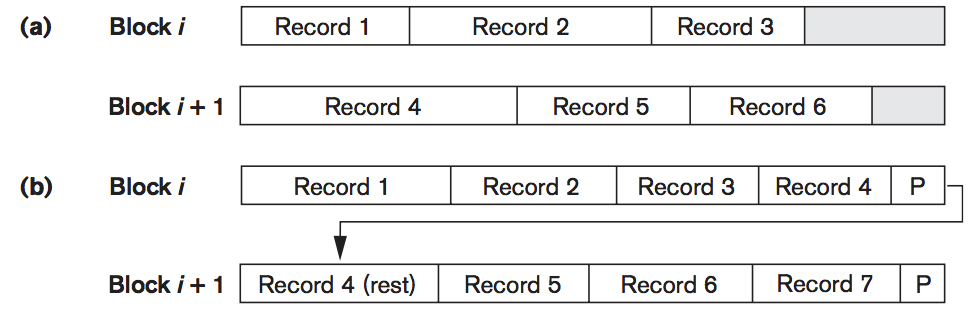
\includegraphics[width=0.7\textwidth]{images/spanned-unspanned}
\end{center}

In any case it is undersirable to have the record split even if it can be split cleanly because it doubles the amount of work to read or write this record (because every operation is on two blocks). We have no choice if the record is bigger than a block, unfortunately, then we must use spanned organization. 

A second problem is that it is difficult to delete a record in this structure. Either we have to have a way to mark the record as deleted or we overwrite it with some record from somewhere else in the file~\cite{dsc}.

If our initial state is as follows~\cite{dsc}:

\begin{center}
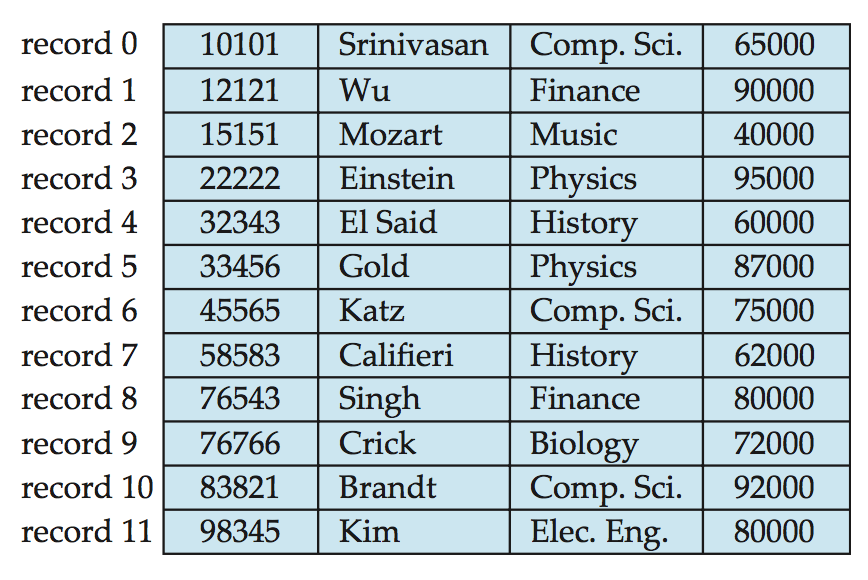
\includegraphics[width=0.4\textwidth]{images/instructor-1}
\end{center}

And we choose to delete record 3, we can either (1) move each record up by one in the file to fill in that gap (left side in the diagram below); or (2) move the last record to fill in that space (right side in the diagram below). Both diagrams from~\cite{dsc}:

\begin{center}
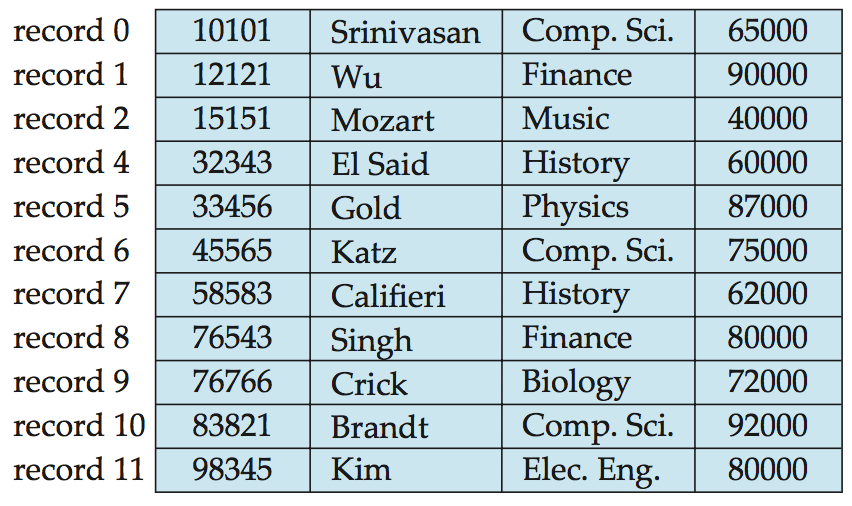
\includegraphics[width=0.4\textwidth]{images/instructor-2} 
~~~~~~~~~~
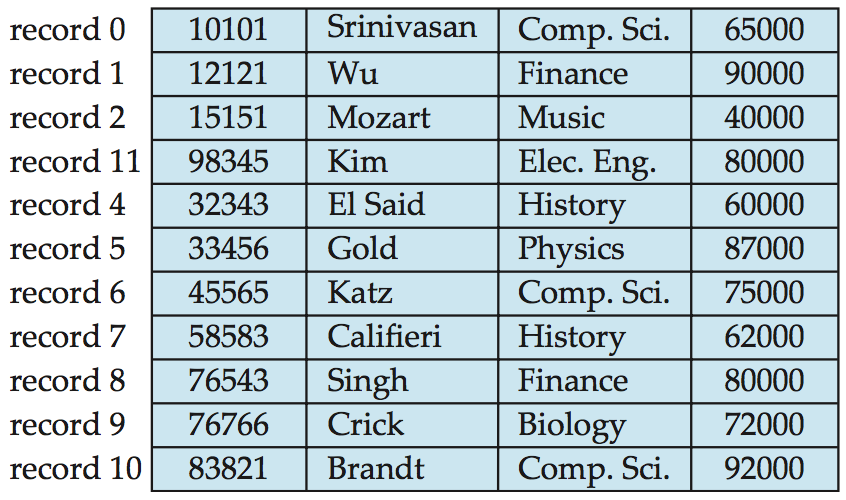
\includegraphics[width=0.4\textwidth]{images/instructor-3}
\end{center}

The first approach requires significantly more work than the second: we have to continually copy each record and overwrite the previous one, potentially $n-1$ times for a block containing $n$ records when the first one is deleted. If we move the last record into the open space it is less work but we still had to copy some data around. We could instead just mark that space as empty. 

Marking the space as empty, however, has its own tradeoffs. If we want to insert a new record then we would have to scan through the whole block to see if there are any empty spaces. Instead of that, we might have a header structure in the file that tells us where the free sections are, if any, in a simple linked list or bitmap structure~\cite{dsc}. 

Of course, things get complicated when we want to insert or delete records that are not fixed length. If we deleted record 3 in the previous example, what do we do if record 11 is bigger than record 3 was? What if it was smaller? We clearly need a different strategy for variable length records.



\paragraph{Variable-Length Records.}

As long as one field is of variable length then we have variable-length records in our file. There are some other situations that might cause record length to vary~\cite{fds}: repeating fields, optional fields, or even putting multiple types of record in the same file. 

A repeating field is one that may have multiple attributes, such as an array of values. This seems strange at first glance since normally one might wish to have a separate relation to represent the array... On the other hand, if it is just a series of strings that might not be sensible. So a customs declaration with a list of clearance document numbers could have the array inside the declaration relation, or in a separate one.

Optional fields are not recommended. If fields are variable length, i.e., not fixed length, then an empty field does not take up any space and it isn't any problem. So let us perhaps leave that subject alone. 

However the variable-length records are implemented, there are two operations we need to consider: (1) how to get records out of a block and (2) how to get particular attributes from a record~\cite{dsc}. Because databases are for retrieval as well as storage we do need an efficient way to get data out again when we want it.

Variable length attributes are often represented in one of two ways. The first is a terminator character of some sort, something not normally allowed in the domain. The next is the attribute is prefixed with its length. If these options sound familiar, they should, because they are the same ways programming languages might represent a variable length string. As you will know, C chose the terminator approach (null-terminated strings) and other languages like Pascal chose the length prefix approach.

The sample layout structure from~\cite{dsc} suggests that fixed length attributes are put together, then each variable length record has an entry of \textit{(offset, length)}  to explain where the variable length attribute is in the file. If the attributes ID, name, and dept\_name in the previous example are variable length, and we have a fourth attribute of fixed length, salary (so it does have leading zeros!) then the length of the record can be computed. For the variable length record, if offset and attribute are 2 bytes each, then we have 4 bytes ``overhead'' per variable length attribute and we get something that looks like this~\cite{dsc}:

\begin{center}
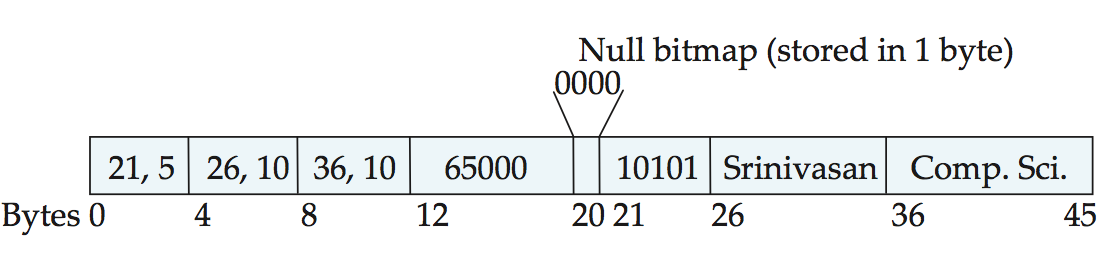
\includegraphics[width=0.7\textwidth]{images/variable-length-record}
\end{center}

The null bitmap (stored in one byte here), tells us which if any of the attributes have a null value. That is one approach to show what values are null; if a value is null when queried then there is no need to actually look at the stored data. The null bitmap could be stored at the beginning or it may not even appear at all: if an attribute is null its length can be zero and that is enough to know there's no data there. It may be a performance improvement to look at the null bitmap and decide if the rest of the data needs to be examined.

Then how do we put the variable length records into a block? For that, the strategy is the \textit{slotted page structure}: a data structure header in each block. The header includes the number of records in that block, where free space ends, and then an array with the location and size of each record. This diagram shows what this looks like~\cite{dsc}:

\begin{center}
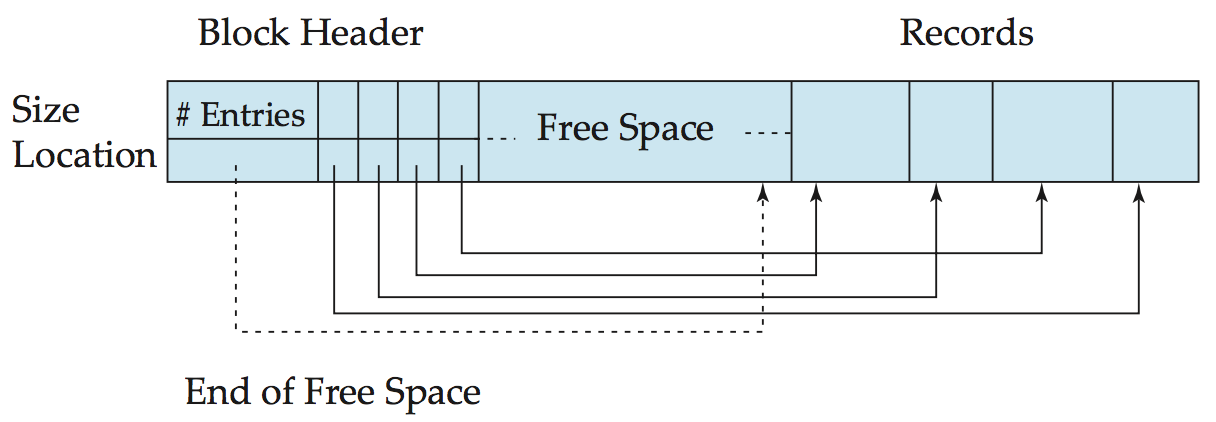
\includegraphics[width=0.7\textwidth]{images/slotted-page}
\end{center}

Records themselves are contiguous in the block and free space exists, perhaps counter-intuitively, between the end of the array and the first record. When a new record is added, it goes at the end of free space and the array gets a little bit bigger (so the free space is reduced at both ends)~\cite{dsc}. 

Deletion requires a bit more work: if an entry is deleted the data is removed and any records between that record and the free space area are moved so that all free space remains contiguous. If a record needs to grow or shrink due to an update statement, then we have to repeat the same procedures and move the records around to ensure that all free space remains contiguous~\cite{dsc}. 

Reorganization following deletion does not have to take place immediately; it is possible to do periodic reorganization when it is a convenient time.

\paragraph{Performance Considerations.}

We can see that there are performance implications for whatever implementation strategy we choose. Performance is not our primary consideration at the moment, nor is it a major focus of this course. However, it is a subject we will want to look at and think about on a regular basis. 

 A select statement can take longer for certain requests than others; if a record is in one block it doesn't take as long to retrieve it as it would if it is spanning two blocks. A seemingly simple update statement may take a different amount of time based on how many records need to be moved if variable allocation is used. If record sizes are fixed then assigning a value may take a constant amount of time... but the number of blocks we need to access to perform an update may be higher because fewer records fit in a block due to all the space being held in reserve for empty values that have not been filled.




\bibliographystyle{alphaurl}
\bibliography{356}


\end{document}
